\documentclass[11pt,letterpaper]{article}
\usepackage{geometry}
\geometry{margin=1in}
\usepackage{graphicx}
\usepackage{float}

\setlength{\parindent}{0pt}
\setlength{\parskip}{0.5em}

%make lists tighter
\usepackage{enumitem}
\setlist{nolistsep}

%reduce spacing before and after section
\usepackage{titlesec}
% reduce section, subsection, etc spacing
\usepackage{titlesec}
\titlespacing*{\section}{0pt}{0\baselineskip}{0\baselineskip}
\titlespacing*{\subsection}{0pt}{0\baselineskip}{0\baselineskip}
\titlespacing*{\subsubsection}{0pt}{0\baselineskip}{0\baselineskip}

%reduce list spacing
\usepackage{enumitem}
\setlist{nosep}

\usepackage[hidelinks]{hyperref}

\title{Lab 2 - Cloud Data, Stat 214, Spring 2025\vspace{-2em}}

% submission must not contain any of your names
% but feel free to make a version for yourself with your names on it
% \author{Your names}

\begin{document}
\maketitle
\section{Introduction}
Each year, human based emissions release more carbon dioxide into Earth’s atmosphere than natural processes can remove, which has caused a massive increase in the amount of carbon dioxide circulating in the atmosphere. In 2023, the global average carbon dioxide was at a record high: 419.3 parts per million (NOAA 2023). Sensitivity of Earth’s climate to the rising levels of atmospheric carbon dioxide is of great interest to the general public and scientific community. Climate models predict that carbon dioxide levels will double within the twenty-first century, which will have especially dire effects in the Arctic. The Arctic region is predicted to be the region where atmospheric carbon dioxide levels will affect the air temperature the most. In order to investigate this, it is essential to gather accurate metrics such as cloud coverage in the Arctic, as the cloud mask is a relevant input to climate models. Clouds keep thermal heat near the Earth’s surface, while reflecting the sun’s radiation back to space. However, it is difficult to get accurate cloud coverage data in the Arctic, since snow, ice and clouds all have similar remote sensing characteristics. 

Typical Satellite images discern objects of interest based on color and temperature. These images are not as useful in the polar regions because all surfaces are white and cold. Instead, the Multi-angle Imaging SpectroRadiometer (MISR) sensor is particularly useful. Unlike traditional single view sensors, MISR takes electromagnetic radiation measurements from nine different cameras positioned at different angles (could include the figure here). MISR allows for better detection of clouds in polar regions because its multi-angle imaging capability helps distinguish between clouds and bright surfaces like ice and snow, reducing misclassification errors that commonly affect single-angle sensors. This report evaluates the efficacy of cloud detection algorithms in the polar regions built on radiance data collected from the MISR sensor. 

\section{EDA}
\subsection{Feature Exploration}
The dataset examined includes 164 MISR images of the polar region. Of these images, only 3 contain ‘expert’ labels discerning clouds and ice sheets. It is difficult to get additional expert labels consistently due to the size of the dataset and the time constraint of manually going through millions of pixels. To circumvent the lack of labeled data, we incorporate transfer learning into our methods to take advantage of the 161 unlabeled images in our training dataset. The three labeled MISR images are displayed below in Figure 1. 

\begin{figure} [H]
    \centering
    
\includegraphics[width=1\linewidth]{expert_label.png}
    \caption{Expert Labels for Cloud Coverage in the Arctic Region}
    \label{fig:enter-label}
\end{figure}

\vspace{1cm}

As shown in Figure 1, even expert labeled data cannot fully classify clouds vs the rest of the polar region. Expert labels are only assigned to pixels where the expert is highly confident in the classification, resulting in many pixels that are left unlabeled. In all three labeled images, there are many pixels that are left unclassified. In Shi et al, the expert labels covered 71.5 percent of valid pixels in their labeled dataset. 

For each pixel, the MISR data includes 5 different radiance angles: DF, CF, BF, AF, and AN. Figure 2 provides a reference how what each of these angles capture. It is natural to examine the relationships between these radiances when examining the same pixels. Table 1 shows the sample correlation between the different radiance angles based on the expert-labeled data. There is a positive correlation for all radiance angles (> 0.59), and some angles display a very strong positive correlation: CF and BF (0.936), BF and AN (0.943), and AN and AF (0.987). 

\begin{table}[H]
\centering
\caption{Sample correlation between the different radiance angles}
\renewcommand{\arraystretch}{1.25}
\begin{tabular}{|c|c|c|c|c|c|}
\hline
Radiance Angles & DF & CF & BF & AF & AN\\ \hline
DF & 1 & .888 & .741 & .636 & .597 \\ \hline
CF & .888 & 1 & \textbf{.936} & .863 & .826 \\ \hline
BF & .741 & \textbf{.936} & 1 & .972 & \textbf{.943} \\ \hline
AF & .636 & .863 & .972 & 1 & \textbf{.987} \\ \hline
AN & .597 & .826 & \textbf{.943} & \textbf{.987} & 1 \\ \hline
\end{tabular}
\end{table}

To distinguish clouds from snow in polar regions, we utilize MISR’s multi-angle radiance data along with three key features derived from Shi, Yu, Clothiaux, and Braverman: CORR, SD, and NDAI. CORR (Correlation of MISR images from different viewing angles) measures the similarity of radiance values across multiple MISR cameras, with high correlations expected over cloud-free surfaces and low-altitude clouds, while high-altitude clouds typically show lower correlations due to scattering differences. However, smooth, cloud-free surfaces such as snow-covered terrain can also exhibit low correlation values due to instrument noise, leading to potential misclassification. To mitigate this, SD (Standard Deviation of nadir-viewing radiance) helps differentiate smooth surfaces by identifying areas with low variability, where low correlation values are more likely due to noise rather than actual cloud presence. NDAI (Normalized Difference Angular Index) quantifies the variation in radiance across different MISR viewing angles, capturing structural differences between clouds and the underlying surface. By combining these three features with MISR’s radiance data, we improve cloud classification accuracy, particularly in challenging polar regions where bright surfaces can otherwise be misclassified as clouds.

\begin{figure}[H]
    \centering
    
\includegraphics[width=1\linewidth, height=1.3\textheight, keepaspectratio]{cloudcorrelations.png}
    \caption{Correlation Matrix of the Features}
    \label{fig:enter-label}
\end{figure}

Figure 2 examines the differences in the correlations between radiance angles and other features in both classes (cloud, no cloud). None of the radiance angles have a negative correlation to each other, which makes sense. The strength of correlation between radiance angles for pixels classified as not cloud was stronger than pixels classified as cloud. The relationships between angles did not seem to deviate too significantly when comparing the two classes. However, when comparing the radiance angles to the derived features, there are several relationships that deviate between the two classes. The relationships between CORR and radiance angles AN, AF and BF are stronger in the cloud class. Additionally, NDAI has a stronger negative correlation to radiance angles AF and BF in the cloud class. 

\subsection{Data Training Split and Data Cleaning}
To ensure that our cloud detection algorithm generalizes well to unseen data, we split our dataset into training and test sets while maintaining spatial variability across different images. Each of the three labeled images is divided into four quadrants, with three quadrants used for training and one reserved for testing. This approach ensures that the training set includes diverse pixel values across different regions, while the test set remains independent to evaluate performance on an unseen portion of the same image. To further prevent data leakage, we excluded pixels near the boundaries of the split quadrants to ensure that adjacent pixels from the same image do not appear in both training and validation sets. Nearby pixels in satellite imagery are highly correlated, and without this separation, the model could learn local spatial patterns rather than generalizable cloud features, leading to overly optimistic performance estimates. We implemented three-fold cross-validation over the training set. The training data was divided into three folds, and within each fold, two subsets were used for training while the last was reserved for validation. The data within each subset originated from the same image to further prevent data leakage during cross-validation. This method of cross-validation mitigates the risk of overfitting to specific spatial patterns that may be present in our small set of training data. 

This method reflects real-world challenges, where cloud detection models need to generalize across different spatial regions rather than overfitting to unique patterns in a single image. Ideally, we would have a larger set of labeled images to train our data on, but using patches allows us to increase the size of our test set while still allowing for some variability in our test set. In future applications of our cloud detection algorithm, the images that we attempt to classify will be different from the dataset that we trained on. To make our model as robust as possible, having an extensive validation procedure is essential. 

In terms of data cleaning, there were no missing values were found so no imputations were needed. As for the unlabeled pixels in the labeled images, they were removed because there was no reasonable way to impute values for them, especially considering that even an expert could not identify the pixel. 

\section{Feature Engineering}
\subsection{Most Important Features}
Assuming that the data are accurate, the training data was scaled and used to train a decision tree model, a random forest model and an gradient boosting model. The mean decrease in impurity for each of the 8 features was computed to quantitatively evaluate the importance of each feature. The training data was also used to train a logistic regression with L2 regularization. Figure 3 shows the bar graph of the logistic regression coefficients for each feature. Figure 4 shows the bar graph of feature importance in each the three tree methods. 

\begin{figure}[H]
    \centering
    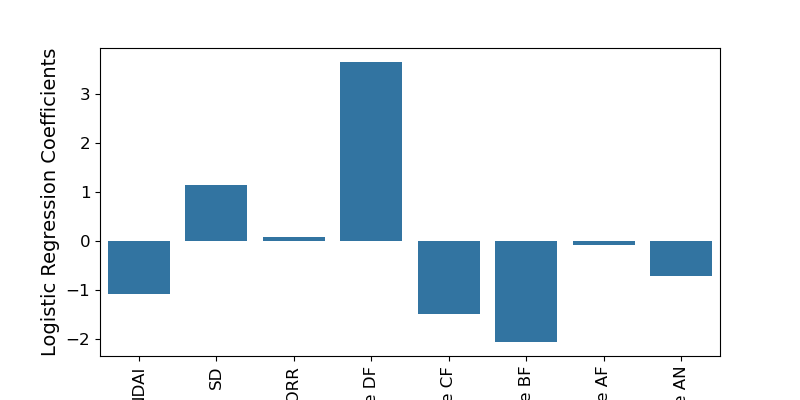
\includegraphics[width=0.75\linewidth]{logreg_coeff.png}
    \caption{Coefficients from logistic regression with an L2 penalty}
    \label{fig:enter-label}
\end{figure}

\begin{figure}[H]
    \centering
    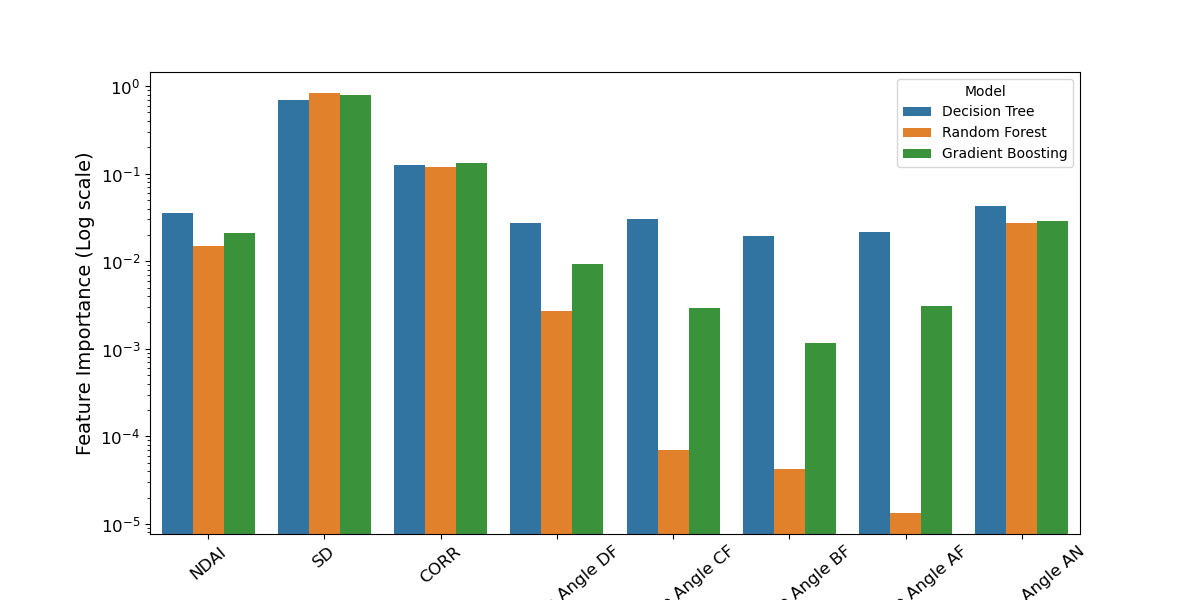
\includegraphics[width=1\linewidth]{feature_importance.png}
    \caption{Mean decrease in impurity for different features}
    \label{fig:enter-label}
\end{figure}

The importance of the features were ranked, from most important to least important, for each model. For the logistic regression coefficients, the absolute value of the coefficients were ranked from the largest to smallest. Then, the rankings for each model were aggregated to obtain a final ranking of feature importance. Table 2 displays the rankings of the different features in different models from most important (1) to last important (8). We take the average ranking to determine the three most important features. 

\begin{center}
\begin{table}[H]
\centering
\caption{Feature importance score rankings from different models}
\renewcommand{\arraystretch}{1}
\begin{tabular}{|c|c|c|c|c|c|}
\hline
 & Decision Tree & Random Forest & Gradient Boost & Logistic Regression & Average \\ \hline
SD & 1 & 1 & 1 & 4 & 1.75 \\ \hline
CORR & 2 & 2 & 2 & 7 & 3.25 \\ \hline
Angle AN & 3 & 3 & 3 & 6 & 3.75 \\ \hline
NDAI & 4 & 4 & 4 & 5 & 4.25 \\ \hline
Angle DF & 6 & 5 & 5 & 1 & 4.25 \\ \hline
Angle CF & 5 & 6 & 7 & 3 & 5.25 \\ \hline
Angle BF & 8 & 7 & 8 & 2 & 6.25 \\ \hline
Angle AF & 7 & 8 & 6 & 8 & 7.25 \\ \hline
\end{tabular}
\end{table}
\end{center}

Based on the feature importance score and rankings, it is clear that SD, CORR, and Radiance Angle AN are the three most important features for classification. The three tree based methods have similar rankings but the logistic regression gives fairly different rankings. We can see from Figure 3 that Radiance Angle DF has a large positive coefficient and Radiance Angle CF and BF have large negative coefficients. This may be due to the fact that many of the variables are highly correlated with one another. For radiance variables in particular, the coefficients have a high variance. This makes the rankings for the logistic regression less trustworthy. However, the difference in the ranking was not enough to outweigh the consensus from the tree-based methods that SD, CORR, and Radiance Angle AN are the three most important features. Figure 5 plots the three most important features along with the expert labels.

\subsection{Engineering New Features}
Using the information from the previous section, new features were created from the three most important features for classification. The 8 features that were provided in the dataset all encode information about the pixel itself and does not use any information from surrounding pixels. So, a new set of features were created to take advantage of the information contained in surrounding pixels. Since SD, CORR, and Radiance Angle AN were the three most important features, we focused on the value of those features in the surrounding pixels. The mean of the SD, CORR, and Radiance Angle AN in the surrounding pixels were calculated for each pixel and were used as three new features in our dataset. These features are named AVG SD, AVG CORR, and AVG AN, respectively.

\begin{figure}[H]
    \centering
    
\includegraphics[width=1\linewidth]{important_features.png}
    \caption{The three most important features and the expert label}
    \label{fig:enter-label}
\end{figure}

\subsection{Transfer Learning}
In addition to standard feature engineering, transfer learning was used to create extra features for the cloud classification model. An autoencoder is trained using unlabeled data, and the values in the latent space of the autoencoder will become new features to be used in our model.

At first, we considered a linear neural network for the encoder, which would be the simpler and less computationally expensive option. However, we ultimately decided to switch to a convolutional neural network to take advantage of the fact that we are working with image data. This means that the autoencoder can better learn local regions of the input, creating features that in theory reflect the patterns better.

\begin{figure}
    \centering
    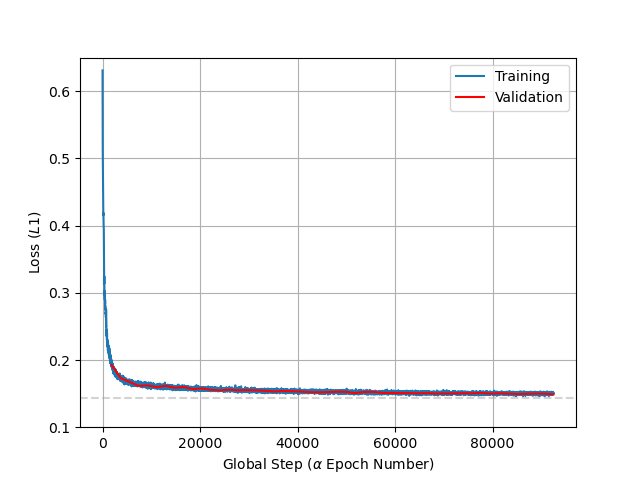
\includegraphics[width=0.75\linewidth]{train-val-loss-against-epochs.png}
    \caption{Autoencoder Loss}
    \label{fig:enter-label}
\end{figure}

We opted for a 5-layer deep network, optimize with respect to $l1$ loss. We decided to use $l1$ loss to encourage sparsity in the embeddings. We got fairly steady results after 50 epochs, as shown in Figure 6, so we set this as a maximum when training the encoder. We used a learning rate of 0.001 and an embedding size of 16 to allow the autoencoder features to learn a more detailed representation. We also tried an embedding size of 8, but our resulting features were not adequate to minimize loss when applying them to our predictive models.




\section{Modeling}
\subsection{Prediction Models}
Using the original features, the engineered features, and the features obtained from the autoencoder, several different classifier models were trained. A logistic regression model, a decision tree model, and a gradient boosting classifier model were trained with varying hyperparameters. The cross-validation F1 score was used to evaluate the performance of these models.


\subsubsection{Logistic Regression}
The first class of models we trained were logistic regression models, which estimate the log odds of a particular label as a linear function of the input features. This approach relies on several assumptions: that observations are independent and identically distributed (i.i.d.), that there is no multicollinearity among features, and that the log odds have a linear relationship with the features. However, in our case, the i.i.d. assumption is violated due to strong correlations between adjacent pixels. To address the high correlation among some features and ensure numerical stability, we applied an L2 regularization penalty.

\begin{center}
\begin{table}[H]
\centering
\caption{Logistic regression F1 score vs L2 regularization strength}
\renewcommand{\arraystretch}{1.25}
\begin{tabular}{|c|c|c|}
\hline
C value &  F1 Score \\ \hline
1 & .758 \\ \hline
0.1 & .779 \\ \hline
0.01 & .791 \\ \hline
0.001 & .801 \\ \hline
\end{tabular}
\end{table}
\end{center}

Four logistic regression models were trained under a L2 regularization penalty, each with a different value of $C$. Table 3 shows the F1 scores of logistic regression models trained with varying values of the regularization parameter C, where smaller values correspond to stronger L2 regularization. As the C value decreases from 1 to 0.001, the F1 score steadily improves from 0.758 to 0.801. This suggests that stronger regularization leads to better model performance by reducing overfitting caused by correlated features and improving generalization.

\subsubsection{Decision Tree}
The second class of models we trained were decision tree classifiers. Decision trees operate by recursively partitioning the feature space using a series of binary thresholding decisions, effectively sorting data points into discrete bins based on their feature values. As a nonparametric method, decision trees do not assume any particular distribution for the input features or residuals. However, they do rely on the assumption that the training data are representative of the data the model will encounter in the future. Since tree-based models do not generalize well beyond the range of the training data, this assumption is critical. In our case, the assumption is reasonable because we treat the labeled dataset as a representative sample of the broader unlabeled dataset. 

\begin{center}
\begin{table}[H]
\centering
\caption{Decision tree F1 score vs maximum depth}
\renewcommand{\arraystretch}{1.25}
\begin{tabular}{|c|c|c|}
\hline
Maximum Depth &  F1 Score \\ \hline
None & .754 \\ \hline
64 & .789 \\ \hline
16 & .804 \\ \hline
\end{tabular}
\end{table}
\end{center}

Three decision tree models were trained, each with a different maximum depth. Table 4 shows the cross-validation F1 score for these models. Based on Table 4, it is evident that shallower decision trees have a better performance. This makes sense in the context of our small training dataset. A shorter tree likely generalizes better to the larger unlabeled dataset. 

\subsubsection{Gradient Boosting Classifier}
The final class of models we trained were gradient boosting classifiers. These models combine the outputs of many shallow decision trees, trained sequentially, where each tree is designed to correct the errors of the previous one by minimizing the loss function. Like other tree-based models, gradient boosting does not extrapolate well beyond the training data, so it assumes that the training and future data are drawn from similar distributions. In our case, this assumption is reasonable given that the labeled data is considered representative of the full dataset.

Three gradient boosting tree models were trained, each with a different number of leaves per tree. Table 5 shows the cross-validation F1 score for these models.

\begin{center}
\begin{table}[H]
\centering
\caption{Gradient boosting tree F1 score vs number of leaves}
\renewcommand{\arraystretch}{1.25}
\begin{tabular}{|c|c|c|}
\hline
Number of Leaves &  F1 Score \\ \hline
15 & .866 \\ \hline
31 & .869 \\ \hline
63 & .870 \\ \hline
\end{tabular}
\end{table}
\end{center}

We trained three gradient boosting models, varying the number of leaves per tree to evaluate the impact of model complexity. Table 5 shows the cross-validated F1 scores for each configuration. As shown in Table 5, increasing the number of leaves per tree led to modest improvements in F1 score. Although overly complex models can overfit the training data, we did not observe overfitting in this case- though this likely would happen if we continued to increase the number of leaves in the model. 

\subsection{Final Model Selection}
The gradient boosting classifier with num\_leaves = 63 was chosen as the final model since the cross validation F1 score for this model (0.870) was higher than that of the logistic regression (0.801) and decision tree classifiers (0.804). After training this model with the entire training set, it had an F1 score of 0.944, an accuracy score of 0.985, a precision of 0.914, and a recall of 0.977 with the test set.

\begin{figure}[H]
    \centering
    
\includegraphics[width=.75\linewidth]{validation_loss_lgbm.png}
    \caption{Validation loss of the model on the test set during training}
    \label{fig:enter-label}
\end{figure}

Figure 7 shows the log loss on the test set across boosting iterations. The loss converges after approximately 60 iterations, stabilizing at a value of 0.044. This indicates that the model successfully converged and additional boosting rounds would not significantly improve performance.

To interpret the model, we evaluated feature importance using the split importance score, which reflects how frequently a feature is used to split the data across all decision trees. A higher split importance score indicates greater influence on the model’s decisions. Figure 8 shows the split importance score of each feature. The features starting with 'ae' indicate that the features are from the embeddings from the autoencoder. Based on the figure, it appears that the features from the autoencoder were the most important features. AVD SD, one of the engineered features, proved to be a fairly important feature as well. Surprisingly, CORR, which was a very important feature prior to feature engineering, turned out to be one of the least important features in our final model. This could be because the autoencoder features may contain the same information as CORR, making the original feature redundant.

\begin{figure}[H]
    \centering
    
\includegraphics[width=0.75\linewidth]{lgbm_feature_imp.png}
    \caption{Split importance score of feature}
    \label{fig:enter-label}
\end{figure}

\subsection{Post Modeling EDA}
After training the model, we classified the images to compare our predictions to the expert labels. Figures 9, 10, and 11 show the expert classified labels vs the predicted labels using our model. The white space between pixels represent the unlabeled pixels from the original image.

\begin{figure}[H]
    \centering
    
\includegraphics[width=1\linewidth]{predicted_label1.png}
    \caption{Expert label vs predicted label, labeled image 1}
    \label{fig:enter-label}
\end{figure}

\begin{figure}[H]
    \centering
    
\includegraphics[width=1\linewidth]{predicted_label2.png}
    \caption{Expert label vs predicted label, labeled image 2}
    \label{fig:enter-label}
\end{figure}




\begin{figure}[H]
    \centering
    
\includegraphics[width=1\linewidth]{predicted_label3.png}
    \caption{Expert label vs predicted label, labeled image 3}
    \label{fig:enter-label}
\end{figure}

For labeled images 1, 2, and 3, the top left, bottom right, and top right quadrants were used as the test data, respectively. There are some visible differences in the prediction accuracy between those regions and the rest, especially labeled image 2. These discrepancies stem from the model being trained on this subset of the image, resulting in localized overfitting to the training data. However, this is expected due to the nature of model training. However, based on the high prediction scores overall, this model still performs well.

Based on the figures, the prediction model works fairly well. However, it tends to misclassify pixels that are on the border between different labels. Based on the lower precision score of the model, the model tends to falsely classify the "Not Cloud" pixels as "Cloud" pixels. This is a common problem in binary classification tasks where there is a gradual transition between classes rather than a clear switch between labels. The model tends to classify the presence of clouds at a higher frequency than experts (a high false positive rate). 

Despite these limitations, the model performs well overall, as indicated by strong evaluation metrics (F1 = 0.944, Accuracy = 0.985, Precision = 0.914, Recall = 0.977). The overall visual alignment between expert and predicted labels further supports the model's generalization ability in labeled regions. 

Next the differences in the distribution of the features in the misclassified and correctly classified pixels were examined. The three most important features identified in section 2 (SD, CORR, Radiance Angle AN) there distributions were plotted in Figures 12, 13, and 14. Based on these figures, there is a stark difference in the distribution of the features between the misclassified and the correctly classified pixels. In particular, misclassified pixels tend to have a higher SD, a higher CORR, and a lower Radiance Angle AN.

\begin{figure}[H]
    \centering
    
\includegraphics[width=1\linewidth]{sd_hist.png}
    \caption{Distribution of SD values}
    \label{fig:enter-label}
\end{figure}

\begin{figure}[H]
    \centering
    
\includegraphics[width=1\linewidth]{corr_hist.png}
    \caption{Distribution of CORR values}
    \label{fig:enter-label}
\end{figure}

\begin{figure}[H]
    \centering
    
\includegraphics[width=1\linewidth]{an_hist.png}
    \caption{Distribution of Radiance Angle AN values}
    \label{fig:enter-label}
\end{figure}

\subsection{Stability Analysis}
Based on the the test loss of the model, and assuming that the labeled images represent the future data well, we expect that the prediction model will work well on unlabeled data. A stability test was performed on the model by training the LightGBM Classifer using a different value for the hyperparameter num\_leaves. Table  6 shows the performance of the new model and compares it with our previously selected model. Figure 15 shows the difference in predictions between the two models. 

Figure 15 and table 6 indicate that the model performs equally well and makes misclassification errors in similar regions. Figure 16 shows the split importance score for each feature in the two models. The feature importance rankings do not change drastically, meaning that the model is fairly stable in this respect as well. 

\begin{center}
\begin{table}[H]
\centering
\caption{Model performances metrics with two different hyperparamters}
\renewcommand{\arraystretch}{1.25}
\begin{tabular}{|c|c|c|}
\hline
 &  num\_leaves=63 & num\_leaves=31 \\ \hline
F1 Score & .944 & .943 \\ \hline
Accuracy & .985 & .985 \\ \hline
Precision & .914 & .911 \\ \hline
Recall & .977 & .978 \\ \hline
\end{tabular}
\end{table}
\end{center}


\begin{figure}
    \centering
    
\includegraphics[width=1\linewidth]{stability_labels.png}
    \caption{Predicted labels using different hyperparameters, num\_leaves=63 (left) and num\_leaves=31 (right)}
    \label{fig:enter-label}
\end{figure}

\begin{figure}[H]
    \centering
    
\includegraphics[width=1\linewidth]{stability_feature_imp.png}
    \caption{Split importance scores using different hyperparameters, num\_leaves=63 (left) and num\_leaves=31 (right)}
    \label{fig:enter-label}
\end{figure}

Lastly, predictions were made on two unlabeled images as a reality check to determine if the model performed differently on the unlabeled data. Figure 17 and 18 show the predicted labels and the Radiance Angle AN side by side for comparison. We chose to use Radiance Angle AN as a reference for the plot of the unlabeled image as it was one of the three most important features in our model. Although these images haven't been labeled by experts, it's generally evident that the model highlights regions that visually resemble clouds.

\begin{figure}[H]
    \centering
    
\includegraphics[width=1\linewidth]{unlabeled_predict1.png}
    \caption{Predicted labels, unlabeled image 1}
    \label{fig:enter-label}
\end{figure}

\begin{figure}[H]
    \centering
    
\includegraphics[width=1\linewidth]{unlabeled_predict2.png}
    \caption{Predicted labels, unlabeled image 2}
    \label{fig:enter-label}
\end{figure}

The figures show some issues in the prediction for pixels with a very low Radiance Angle AN value, which represent land not covered by snow or clouds. However, the predictions in other regions seem reasonable. Overall we were able to create a model that can differentiate between clouds and snowy surfaces well.

\section{Conclusion}
Due to the scarcity of expert-labeled data (3 labeled images of 164 total images), we leveraged both traditional machine learning and transfer learning techniques to improve classification performance. A key component of our approach was the use of a convolutional autoencoder trained on unlabeled data to extract meaningful latent features that capture local spatial and radiometric patterns. These autoencoder embeddings were used alongside original and engineered features as inputs to our predictive models. In our final model, several of the most important features were features extracted from the autoencoder. 

Among the models we tested—logistic regression, decision trees, and gradient boosting- gradient boosting consistently achieved the highest F1 score (0.944) on the test set. Feature importance analysis revealed that the autoencoder-derived features dominated the model's decision-making, indicating that they captured complex patterns in the data that were not encoded in the original radiance features alone. This demonstrates the value of incorporating unsupervised deep learning methods into satellite image analysis pipelines, especially when labeled data is limited. Our final model generalized well across images and offers a promising foundation for scalable cloud detection in polar regions.

Future steps for this work include expanding the labeled dataset to improve model generalization and reduce local overfitting. Because we only trained on three images, we split the images up into patches to train and validate our model. Especially in regions where prediction accuracy varies across image quadrants, more labeled data would allow for increased generalization of our model.

\section{Bibliography}
NOAA Climate.gov. (n.d.). Climate change: Atmospheric carbon dioxide. National Oceanic and Atmospheric Administration. https://www.climate.gov/news-features/understanding-climate/climate-change-atmospheric-carbon-dioxide

Shi, T., Yu, B., et al. (2008). Daytime Arctic cloud detection based on multi-angle satellite data with case studies. Journal of the American Statistical Association.
\appendix
\section{Academic honesty}
\subsection{Statement}
We designed and performed all the data analysis procedures presented in this report. We wrote all the texts and produced all the figures in this report. We have included and documented all the procedures in the workflow and the results can be fully reproduced. We believe that academic honestly is important because it creates a fair environment for everyone, judging us by our true decisions and work ethic, which allows for accurate
representation of industry and research.
\subsection{LLM Usage}


\subsubsection*{Coding}
ChatGPT was used to help understand how the autoencoder works and how to implement different architectures for the autoencoder. It was also used to better understand error messages. We also consulted LLMs to help generate some basic visualizations.
\subsubsection*{Writing}
ChatGPT was not used to write any portion of this report.

\end{document}
